\documentclass{article} % For LaTeX2e
\usepackage{latex_template,times}
\usepackage{hyperref}
\usepackage{url}
\usepackage{euler}
\usepackage{natbib}
\usepackage{amsmath}
\usepackage{prettyref}
\usepackage[]{hyperref}
\usepackage{mathtools}
\usepackage{csvsimple}
\usepackage{booktabs}

\DeclarePairedDelimiter{\norm}{\lVert}{\rVert}
% in dvi it only seems to use urlcolor !!!!
\hypersetup{colorlinks,linkcolor=blue,citecolor=blue,pagecolor=blue,%
            urlcolor=magenta,filecolor=magenta,breaklinks,%
            dvips,bookmarks,bookmarksopen}
%\documentstyle[nips14submit_09,times,art10]{article} % For LaTeX 2.09

%\author{Chen C che5002 480458339, Yutong Cao ycao5602 470347494,***}
\title{Assignment 2}

\newcommand{\fix}{\marginpar{FIX}}
\newcommand{\new}{\marginpar{NEW}}
\newcommand{\svm}{\textsc{svm}}

\nipsfinalcopy % Uncomment for camera-ready version

\begin{document}

\author{%
 \begin{tabular}{rl}
  Tutors: & Zhuozhuo Tu, Liu Liu\\ \\
Group members: & Chen Chen (cche5002) 480458339, \\
& Yutong Cao (ycao5602) 470347494,\\
& Yixiong Fang ***
\end{tabular}
}

\maketitle



\begin{abstract}
The abstract paragraph should be indented 1/2~inch (3~picas) on both left and
right-hand margins. Use 10~point type, with a vertical spacing of 11~points.
The word \textbf{Abstract} must be centred, bold, and in point size 12. Two
line spaces precede the abstract. The abstract must be limited to one
paragraph.
\end{abstract}
\section{Introduction}
This report documents our modification of support vector machine~(\svm) to improve its performance again label noise.

Label noises are unavoidable in many data sets. In probability theory and machine learning, the law of large numbers states that the average of samples drawn converge to the expected value of a random variable with a larger number of trials \citep{hardle2007applied}. Besides the choices of hypothesis class, objective function, optimisation method, and output hypothesis, the size and quality of the data used are also crucial in training a model. 

Most of the data labelling work are done by humans. Thus mistakes can hardly be avoided, especially when the data size and the number of classes are relatively large. Usually there is a trade-off between the data complexity and the data quality. Weakly supervised learning methods are introduced to handle this kind of problems. Positive and unlabelled (\textsc{pu}) learning and semi-supervised learning are designed to trade data complexity for data quality. They both make use of a small set of correct data to train a model. Also there is learning with noisy labels, on the contrary, trades data quality for data complexity. It learns a model with a large amount of noisy data. In this assignment, we only focused on the latter.

We implemented three methods for learning with noisy labels and conducted experiments with them on two noisy data sets. For both data sets, the flip rates are given. Our first method is to learn with a modified support vector machine. The label noise information is added to the optimisation term of the SVM as a function of the observed label and an error term which follows a Bernoulli distribution. This method is first proposed by \citet{pmlr-v20-biggio11} to learn with random classification noise (\textsc{rcn}), and we extended it to learn with class-dependent noise (\textsc{ccn}). The second method is the heuristic approach based on the work of \citet{Wu03probabilityestimates}. This method follows the assumption that models trained with the noisy data still give an adequate performance. Thus the predicted probability of a noisy sample point belonging to one class should be around 0.5 as the model can neither accept nor reject the prediction with confidence. We exclude the potential noisy data points following this idea and train a model on the rest data which we believe are cleaner than the original data. The third method is the importance reweighting approach proposed by \citet{liu2016classification}. This method calculates a reweighting coefficient for each sample point using the result from training a model on the original noisy data to reweight the loss for each sample point. For all three methods, we choose use the same classification model so that we can compare the three learning with label noise methods with the rest conditions controlled. Although \textsc{svm} is not considered to be robust to label noise, its classification accuracy is relatively high compared with other models.

We used the three methods to learn two sets of noisy data, both containing 10,000 instances belongs to two classes. The first data set is sampled from the fashion-mnist database and the second is sampled from the \textsc{cifer} database. We will compare our results from using the three learning with label noise methods on both data sets in accuracy and process time. For all three methods, the values of noise rates are required. We implemented a noise rate estimation using the method proposed in the work of \citet{liu2016classification}. We did not use the estimated values in our classification experiments as the true rates are provided. But we will compare our estimation with the true values.

\section{Related work}
In the literature, there are many works on learning with label noise. One popular approach is to use classification algorithms that are proved to be robust to label noise. \cite{frenay2014classification} summarised in their work that 0-1 loss and least-squares loss are robust loss functions to label noise. Also, bagging and ensemble decision tree are robust classification models to learn with label noise. This kind of approach does not deal with label noise directly. Instead, they treat the noisy sample points as outliers and assume they will not have too much effect on the trained model. We chose not to use the robust loss functions as the corresponding classification models may not produce satisfying classification accuracy as \textsc{svm}. But we used a bagging-like technique by sampling multiple times and averaging the predicted probabilities to generate better and more stable predictions. \cite{frenay2014classification} also mentioned filtering methods for learning with label noise. This kind of methods try to remove mislabelled data before training a final model. Our second model follows this idea by excluding data points with vague predictions. \cite{yang2018adasampling} also proposed a filter-like method that filters the data during training and calculates a mislabelled probability for each sample rather than removing them directly. Many of the approaches mentioned above do not consider the noise rates as known. Although this makes the problem general, the methods may not be able to handle more complicated problems. \\ \\
\citet{pmlr-v20-biggio11} proposed a method that rewrites the objective function and adds the noise rate information to it. They substitutes the given label values with expected values and optimises the new objective function. This is what our first learning with label noise method is based one. The idea behind this method is clear and intuitive, but it is only applicable for certain loss functions. \citet{liu2016classification} proposed an importance reweighting method that reweights the surrogate loss function using information from a pre-train process. This method does not have limitations on the type of surrogate functions chosen. And they also provided an efficient method for estimating the noise rate. 

\section{Method}
We use \textsc{svm} with Gaussian kernel as the base classification method for this task because of its generalisation ability.

\textsc{svm} with Gaussian kernel was first published by \citet{Boser:1992:TAO:130385.130401}. \citet{Cortes1995} an improvement with soft-margin \textsc{svm} to  avoid over-fitting problem. The \textsc{svm} is to minimise the Hinge loss function
\begin{equation*}
\left[{\frac {1}{n}}\sum _{i=1}^{n}\max \left(0,1-y_{i}(w\cdot x_{i}-b)\right)\right]+\lambda \lVert w\rVert ^{2}.   
\end{equation*}
Here, $w$ is the weighting factor, $b$ is a constant. We classify the $i$th image into category~$1$ or~$-1$ when $w\cdot x_{i}-b\geq1$ or $w\cdot x_{i}-b\leq-1$, respectively. This loss function not only penalises points that misclassified, but also points that are closed to the dividing hyperplane, with a regularisation term~$\lambda \lVert w\rVert ^{2}$. \citet{Fernandez-Delgado:2014:WNH:2627435.2697065} suggested \svm\ is very likely to be one of the most powerful classifiers, by comparing 179 classification algorithms over 121 large data sets. The distances between data points and the dividing hyperplane gives an intuitive estimate of the generalisation ability of the trained \svm\ model \citep{hastie01statisticallearning}. 

In this image classification assignment, we do not observe the true labels~$y_i$. This section proposes three different approaches to modify ordinary \svm\ to attack label noise problem. However, we do not have access to a test data set with true labels~$(x_i,y_i)$ to verify the generalisation ability of our three different models, which are all trained by noisy data~$(x_i,S_i)$. Using \svm , the gap between hyperplane and the training data set provides a natural and `free' metric of its generalisation ability  \citep{hastie01statisticallearning}, and also provides an alternative to using a test data set. As of the strong generalisation ability of a well-trained \svm\ \citep{Cortes1995,NIPS2012_4500}, it was chosen as our classification method.
\subsection{Preprocess}
\texttt{StandardScaler} from \texttt{sklearn} was used. Each image is rescaled to have mean zero and standard deviation one. By doing this, we removed the brightness difference among different images. This process is called photometric normalisation. \citet{jonsson2002support} suggested that this may improve the performance of Gaussian kernel SVM as Gaussian kernel is a radius based kernel and hence it performs well when images are on the same scale. For the \textsc{cifer} dataset, we used principle component analysis (\textsc{pca}) for dimension reduction. We did not run \textsc{pca} on the fashion-mnist data because the dimension is reasonable.

\subsection{The original data set is balanced} \label{sec:1}
The assignment instruction states the probabilities~$P(S=1|Y=0)=0.2$ and $P(S=0|Y=1)=0.4$. From the data, we observed that $40\%$ of contaminated labels~$S$ (i.e. $P(S=1)$) is $1$. As a result
\begin{eqnarray*}
P(S=1)&=&P(S=1|Y=1)P(Y=1)+P(S=1|Y=0)P(Y=0)\\
     &=&\left[1-P(S=0|Y=1)\right]P(Y=1)+P(S=1|Y=0)P(Y=0)\\
     &=&0.6P(Y=1)+0.2\left[1-P(Y=1)\right]=0.4, \nonumber
\end{eqnarray*}
which implies $P(Y=1)=P(Y=0)=0.5$ and the original classification problem is balanced.In addition, define the Bernoulli random variable~$\epsilon(S)$ with the means $E(\mu(\epsilon)(S=0))=P(Y=1|S=0)=0.5\times0.4/0.6=1/3$ and $E(\epsilon(S=1))=P(Y=0|S=1)=0.5*0.2/0.4=0.25$. This random variable~$\epsilon$ describe the unobserved random label noise. Hence the expectation is
\begin{equation}
    E\epsilon(S)=P(Y=0|S=1)P(S=1)+P(Y=1|S=0)P(S=0)=0.25\times 0.4+1/3\times0.6=0.3.\label{eq:exp}
\end{equation}
\subsection{Method 1: Modified support vector machine}
We proposed a modified support vector machine (\textsc{svm}) to attack this classification problem with label noise. We describe the mathematical justification for our modification.
%---the given label noise where flip rates~$P(S=1|Y=0)=0.2$ and~$P(S=0|Y=1)=0.4$ seems to be marginally different to a random label noise with flip rate~$P(S=1|Y=0)=P(S=0|Y=1)=0.3$ for \textsc{svm}.
\subsubsection{Expectation maximisation}
This section extends the expectation maximisation algorithm proposed by \citet{pmlr-v20-biggio11}. The original algorithm was proposed to encounter random classification noise where the flip rate $\rho_+=\rho_-$ and we extend it to manage the case dependent label noise where the flip rates $\rho_+\neq\rho_-$.

Recall the dual problem of an \textsc{svm} is to maximise
\begin{equation}
   f(c_{1}\ldots c_{n})=\sum _{i=1}^{n}c_{i}-{\frac {1}{2}}\sum _{i=1}^{n}\sum _{j=1}^{n}y_{i}c_{i}k(x_{i},x_{j})y_{j}c_{j}, \label{eq:dual}
\end{equation}
\begin{math}
{\text{subject to }}\sum _{i=1}^{n}c_{i}y_{i}=0,\,{\text{and }}0\leq c_{i}\leq {\frac {1}{2n\lambda }}\;{\text{for all }}i. 
\end{math} 
Here $y_i$ and $x_i$ are the labels and features of the $i$th image, $c_i$ is the $i$th Lagrangian multiplier, $k(x_i,x_j)$ is the Gaussian kernel product of $x_i$ and $x_j$
\begin{equation*}
\exp(-\gamma\norm{x_i-x_j}).
\end{equation*}
Substitute label noise~$y_i=S_i(1-2\epsilon(S_i))$ into objective function~\eqref{eq:dual}
\begin{equation}
   f(c_{1}\ldots c_{n})=\sum _{i=1}^{n}c_{i}-{\frac {1}{2}}\sum _{i=1}^{n}\sum _{j=1}^{n}S_{i}c_{i}k(x_{i},x_{j})S_{j}c_{j}(1-2\epsilon(S_i))(1-2\epsilon(S_j)), \label{eq:dual2}
\end{equation}
When $i=j$, the expectation~$E(1-2\epsilon(S_i))(1-2\epsilon(S_j))=1-4E\epsilon(S_j)+4E\epsilon(S_j^2)=1$. When $i\neq j$, the expectation~$E(1-2\epsilon(S_i))(1-2\epsilon(S_j))=(1-2E\epsilon(S_i))(1-2E\epsilon(S_j))=1-\mu$ where parameter~$\mu:=0.84$, by substituting expectations~\eqref{eq:exp} from Section~\ref{sec:1}. 

Define kernel correction matrix~$M$ with the $(i,j)$-th entry being $m_{ij}$.The diagonal entries~$m_{ii}=1 $, and the off diagonal entries~$m_{ij}=1-\mu=0.16$ when indexes~$i\neq j$. Using the technique of Expectation maximisation, 
\begin{equation}
   Ef(c_{1}\ldots c_{n})=\sum _{i=1}^{n}c_{i}-{\frac {1}{2}}\sum _{i=1}^{n}\sum _{j=1}^{n}S_{i}c_{i}k(x_{i},x_{j})S_{j}c_{j}m_{ij}, \label{eq:dual3}
\end{equation}
The only difference between our modified \textsc{svm} and ordinary \textsc{svm} is to replace the kernel matrix~$K$ with our new proposed matrix~$Q:=K\circ M$.

\subsubsection{Tuning}
Define data vector~$\vec{x}:=(x_1,x_2,\ldots , x_n)$. The Kernel parameter for Gaussian Kernel~$\gamma$ is chosen to maximise the Variance of Kernel matrix~$K(\vec{x},\vec{x})$. The regularisation parameter is chosen to be one as the model seems to be insensitive to the regularisation parameter.

%\subsubsection{Additional regularisation}


%This soft-margin \textsc{svm} is sub-optimal for our problem. We have a large set of data ($10,000$) comparing with the number of features ($784$). Hence, we build a modified \textsc{svm} that aims to minimise the following Hinge loss
%\begin{equation}
%\left[{\frac {1}{n}}\sum _{i=1}^{n}\max \left(0,10-y_{i}(w\cdot x_{i}-b)\right)\right]+\lambda \lVert %w\rVert ^{2}.   \label{eq:pri}
%\end{equation}
%The modified constant~$10$ requires the predictor~$w\cdot x_{i}-b$ to be as extreme as possible, i.e., it penalises wrongly classified samples. Moreover, it even penalises correctly classified samples with small gaps between data points and the dividing hyper-plane being small. 
%Define $\zeta _{i}:=\max \left(0,10-y_{i}(w\cdot x_{i}-b)\right)$. The prime problem of Hinge loss~\eqref{eq:pri} becomes a minimisation of
%\begin{equation}
%{\frac {1}{n}}\sum _{i=1}^{n}\zeta _{i}+\lambda \|w\|^{2}
%{\text{ subject to }}y_{i}(w\cdot x_{i}-b)\geq 10-\zeta _{i}\,{\text{ and }}\,\zeta _{i}\geq 0,\,{\text{for all }}i. \label{eq:pri2}
%\end{equation} 
%The modification is inspired by observing that the regularisation parameter~$\lambda$ has a negligible impact on the classification results for this problem. Hence we have more than enough data to train this complex model without over fitting.

%The modified \textsc{svm} aims to make the algorithm more robust to label noise, even though it may enlarge the generalisation error. Nevertheless, the large data set will assure us the generalisation error is within a reasonable magnitude.
%The parameters~$c_i$ are Lagrangian multipliers that enforcing the condition~$y_{i}(w\cdot x_{i}-b)\geq 10-\zeta _{i}$ in prime problem~\eqref{eq:pri2}.

%With this modification, the dual problem~\eqref{eq:dual3} of the loss function~\eqref{eq:pri} becomes
%\begin{equation*}
%   Ef(c_{1}\ldots c_{n})=10\sum _{i=1}^{n}c_{i}-{\frac {1}{2}}\sum _{i=1}^{n}\sum %_{j=1}^{n}S_{i}c_{i}k(x_{i},x_{j})S_{j}c_{j}m_{ij}. \label{eq:dual3}
%\end{equation*}
%From the dual prospective, we are weakening the contributions of the contaminated labels~$S_i$, hence making the algorithm more robust.



This method gives us an accuracy of $94.6\%$ on the testing data.

\subsection{Method 2: heuristic approach}
Method 2 still implement \textsc{svm}. We chose \textsc{svm} because classification algorithms with Hinge loss, including \textsc{svm}, is robust against random classification label noise. Our label noise is class dependent. However, experiment shows that \textsc{svm} is still robust against it.
%\subsubsection{Hinge loss is robust against label noise}

\subsubsection{Select samples}
Ordinary \textsc{svm} only gives a classification without revealing a probability that indicates the confidence of classification. \citet{Wu03probabilityestimates} proposed a five-fold cross-validation method to calculate the classification probabilities~$P(Y=1|X_i)$ for \textsc{svm}. 
Using this method, we calculated the probability~$P(Y=1|X_i)$ with label noise by an \textsc{svm} with Gaussian kernel. We have $10,000$ samples. We only use those with largest and smallest $P(Y=1|X_i)$ (first $1/3$ and last $1/3$), because intuitively the contaminated samples are more likely to have a probability~$P(Y=1|X_i)$ close to $0.5$ and the error rate $P(\epsilon=1)=0.3$. A $3\%$ margin was left because classification errors must exist.
\subsubsection{Label correction}
We relabel the $1/3$ of the samples with highest fitted probability~$P(Y=1|X_i)$ as $1$ and the $1/3$ samples with the smallest fitted probability~$P(Y=1|X_i)$ as $-1$. This step is important because section~\ref{sec:1} shows that the original data set is balanced ($P(Y=1)=P(Y=0)=0.5$). 

Training our \textsc{svm} with Gaussian Kernel again with this subset of relabeled data gives our second model.

This method gives us an accuracy of $95.0\%$ on the testing data.
%\subsubsection{Hinge loss if robust against label noise}
\subsection{Method 3: Reweighting}
Please copy some formulae to here from tut11.

\section{Result}
\begin{table}
	\begin{tabular}{lllll}
\hline 
Data & Null Hypothesis ($H_0$) & $D$ & P-value & Reject $H_0$\\
\hline 
\hline 
 & Relabelling algorithm is no more accurate than expectation maximisation.  & 0.625 & 0.0019 & Reject\\
 
 \textsc{mnist} & Expectation maximisation algorithm is as accurate as Reweighting. & 0.3125 & 0.4154 & Fail to reject\\
 
  & Reweighting algorithm is as accurate as relabelling. & 0.3125 & 0.4154 & Fail to reject\\
\hline 
   & Expectation maximisation algorithm is no more accurate than relabelling. & 0.5 & 0.0183 & Reject\\

 \textsc{cifar}  & Reweighting algorithm is no more accurate than expectation maximisation. & 0.6875 & 0.0005 & Reject\\

  & Reweighting algorithm is no more accurate than relabelling.  & 0.6875 & 0.0005 & Reject\\
\hline 
\end{tabular}
	\caption{Hypothesis test}
	\label{tab:HypothesisTest}
\end{table}
\begin{table}
	\caption{Mean sd}
	\label{tab:Meansd}
    \csvautobooktabular[late after head=]{meansd.csv}
\end{table}


\begin{figure}
	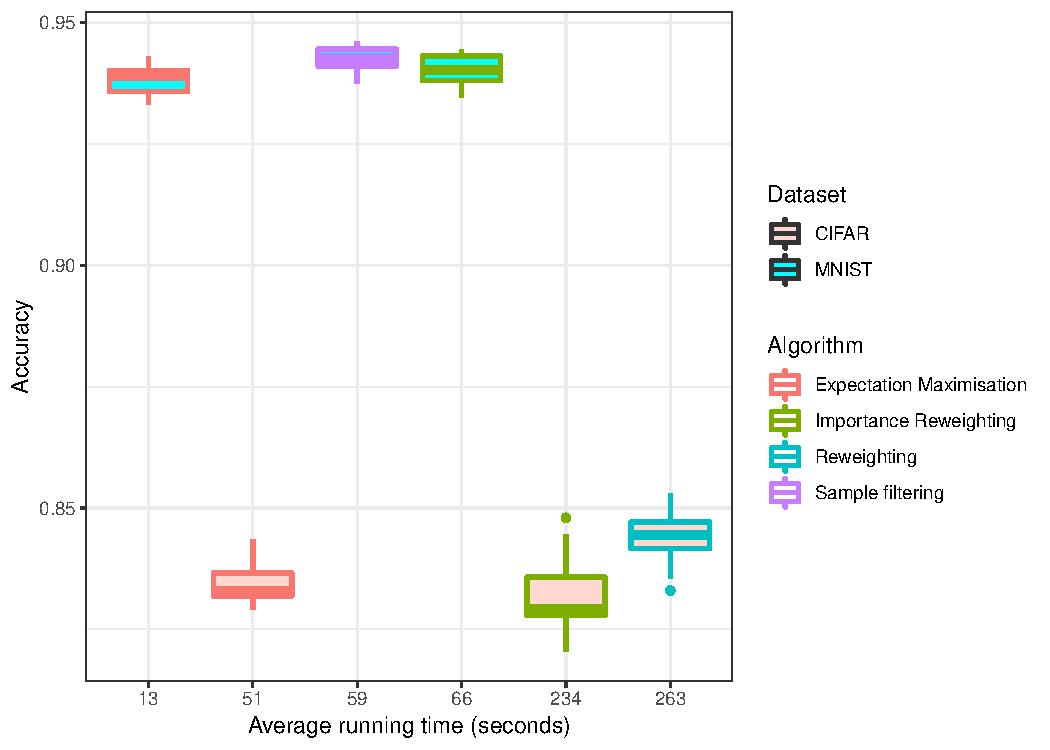
\includegraphics{boxplot.pdf}
	\caption{Boxplot}
	\label{fig:Boxplot}
\end{figure}

\begin{figure}
	 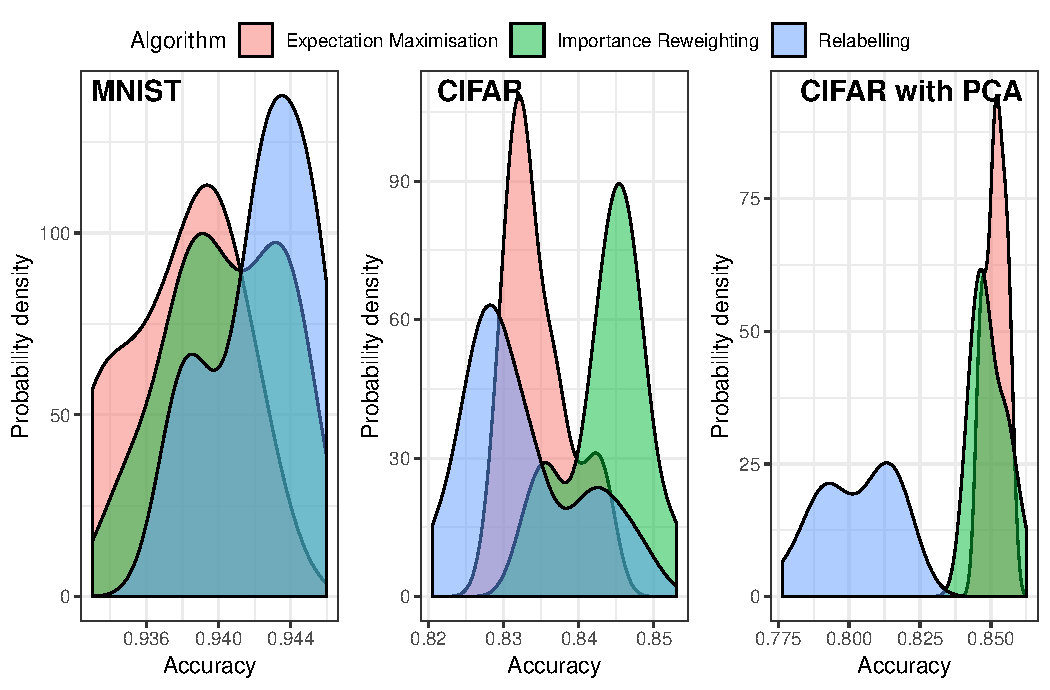
\includegraphics{histo.pdf}
	\caption{Density function from kernel smoothing}
	\label{fig:Density function from kernel smoothing}
\end{figure}

scatter plot of time vs. accuracy
histogram of accuracy
mean, sd table

Please pay special attention to the instructions in section \ref{others}
regarding figures, tables, acknowledgments, and references.

\section{Headings: first level}
\label{headings}

First level headings are lower case (except for first word and proper nouns),
flush left, bold and in point size 12. One line space before the first level
heading and 1/2~line space after the first level heading.

\subsection{Headings: second level}

Second level headings are lower case (except for first word and proper nouns),
flush left, bold and in point size 10. One line space before the second level
heading and 1/2~line space after the second level heading.

\subsubsection{Headings: third level}

Third level headings are lower case (except for first word and proper nouns),
flush left, bold and in point size 10. One line space before the third level
heading and 1/2~line space after the third level heading.

\section{Citations, figures, tables, references}
\label{others}


\subsection{Citations within the text}

Citations within the text should be numbered consecutively. The corresponding
number is to appear enclosed in square brackets, such as [1] or [2]-[5]. The
corresponding references are to be listed in the same order at the end of the
paper, in the \textbf{References} section. (Note: the standard
\textsc{Bib\TeX} style \texttt{unsrt} produces this.) As to the format of the
references themselves, any style is acceptable as long as it is used
consistently.


\subsection{Footnotes}

Indicate footnotes with a number\footnote{Sample of the first footnote} in the
text. Place the footnotes at the bottom of the page on which they appear.
Precede the footnote with a horizontal rule of 2~inches
(12~picas).\footnote{Sample of the second footnote}

\subsection{Figures}

All artwork must be neat, clean, and legible. Lines should be dark
enough for purposes of reproduction; art work should not be
hand-drawn. The figure number and caption always appear after the
figure. Place one line space before the figure caption, and one line
space after the figure. The figure caption is lower case (except for
first word and proper nouns); figures are numbered consecutively.

Make sure the figure caption does not get separated from the figure.
Leave sufficient space to avoid splitting the figure and figure caption.

You may use color figures.
However, it is best for the
figure captions and the paper body to make sense if the paper is printed
either in black/white or in color.
\begin{figure}[h]
\begin{center}
%\framebox[4.0in]{$\;$}
\fbox{\rule[-.5cm]{0cm}{4cm} \rule[-.5cm]{4cm}{0cm}}
\end{center}
\caption{Sample figure caption.}
\end{figure}

\subsection{Tables}

All tables must be centered, neat, clean and legible. Do not use hand-drawn
tables. The table number and title always appear before the table. See
Table~\ref{sample-table}.

Place one line space before the table title, one line space after the table
title, and one line space after the table. The table title must be lower case
(except for first word and proper nouns); tables are numbered consecutively.

\begin{table}[t]
\caption{Sample table title}
\label{sample-table}
\begin{center}
\begin{tabular}{ll}
\multicolumn{1}{c}{\bf PART}  &\multicolumn{1}{c}{\bf DESCRIPTION}
\\ \hline \\
Dendrite         &Input terminal \\
Axon             &Output terminal \\
Soma             &Cell body (contains cell nucleus) \\
\end{tabular}
\end{center}
\end{table}



\subsection{Margins in LaTeX}

Most of the margin problems come from figures positioned by hand using
\verb+\special+ or other commands. We suggest using the command
\verb+\includegraphics+
from the graphicx package. Always specify the figure width as a multiple of
the line width as in the example below using .eps graphics
\begin{verbatim}
   \usepackage[dvips]{graphicx} ...
   \includegraphics[width=0.8\linewidth]{myfile.eps}
\end{verbatim}
or % Apr 2009 addition
\begin{verbatim}
   \usepackage[pdftex]{graphicx} ...
   \includegraphics[width=0.8\linewidth]{myfile.pdf}
\end{verbatim}
for .pdf graphics.
See section 4.4 in the graphics bundle documentation (\url{http://www.ctan.org/tex-archive/macros/latex/required/graphics/grfguide.ps})

A number of width problems arise when LaTeX cannot properly hyphenate a
line. Please give LaTeX hyphenation hints using the \verb+\-+ command.


\bibliographystyle{unsrtnat}
\bibliography{reference}



\end{document}
